% When Structure Hurts: Understanding Evidence Loss in Retrieval-Augmented Reasoning
% ACL format (official acl-org/acl-style-files, commit d5adc823ff0f), anonymous review mode.
% Every number in this paper is read from research_outputs/ (see CLAIMS_EVIDENCE_AUDIT.md).
\documentclass[11pt]{article}
\usepackage[review]{acl}
\usepackage{times}
\usepackage{latexsym}
\usepackage[T1]{fontenc}
\usepackage[utf8]{inputenc}
\usepackage{microtype}
\usepackage{inconsolata}
\usepackage{graphicx}
\usepackage{booktabs}
\usepackage{amsmath}
\usepackage{amssymb}
\usepackage{multirow}
\usepackage{adjustbox}
\usepackage{xcolor}
\usepackage{tikz}
\usetikzlibrary{arrows.meta,positioning}

\title{When Structure Hurts: Understanding Evidence Loss\\in Retrieval-Augmented Reasoning}

% Authorship and affiliations are not set here: they must be confirmed by the authors
% (paper/README.md). Review mode prints "Anonymous ACL submission".
\author{Anonymous ACL submission}

\begin{document}
\maketitle

\begin{abstract}
Retrieval-augmented systems increasingly turn retrieved passages into sentence lists, reasoning orders and relation graphs before generation. System-level comparisons cannot tell which part of such a transformation helps or hurts, because retrieval, content and formatting change together. We hold the evidence fixed: gold supporting passages for multi-hop questions are presented in representations whose fact sets are verified identical per question, and we vary segmentation, order, relation lines and their labels one at a time. In a pre-specified test on 4{,}976 MuSiQue and 2WikiMultiHopQA questions with Qwen2.5-7B-Instruct, graph-derived ordering and derived relation lines had no detectable effect, and splitting passages into sentence items lowered 2WikiMultiHopQA exact match by 1.7 points, through abstention; the latter did not replicate with Mistral-7B. Exploratory fixed-order interventions then located the cost of predicted structure in a single label: showing the \texttt{CONTRADICTS} relations predicted by an NLI classifier cost about 3 points, and relabelling only those lines recovered it. A second pre-specified test on 6{,}400 untouched questions confirmed the effect (2WikiMultiHopQA $-7.7$ points, HotpotQA $-5.3$ points among affected questions), mostly through abstention and partly through wrong answers; it also held for Mistral. Whether the harmful contradictions are false is supported only by automatic triage, and all results concern 7B readers.
\end{abstract}

\section{Introduction}
\label{sec:intro}

Retrieval-augmented generation (RAG) gives a language model access to text that its parameters do not contain, by retrieving passages and placing them in the prompt \citep{lewis2020rag}. For questions that require combining several facts, as in multi-hop benchmarks such as MuSiQue, 2WikiMultiHopQA and HotpotQA \citep{trivedi2022musique,ho2020twowiki,yang2018hotpotqa}, the passages are typically handed to the model as an unordered list and left for the model to link.

A growing family of methods therefore transforms retrieved evidence before generation. Passages are decomposed into propositions or atomic claims \citep{chen2024densex}, organised into trees of summaries \citep{sarthi2024raptor}, or linked into entity and fact graphs whose nodes, relations and paths are serialised into the prompt \citep{edge2024graphrag,gutierrez2024hipporag,gutierrez2025hipporag2,zhu2025kg2rag,guo2024lightrag,chen2026pathrag}.

Every such transformation can also go wrong. An extractor may omit the sentence that names the answer, and a token budget may cut it because the structured format spends tokens on identifiers and relation lines. Splitting a passage into sentences turns ``It stars Anne Hathaway \dots'' into an item whose subject must be recovered from elsewhere. A relation predictor may add a statement that the source never made: in our experiments, it marked ``The teaser of the film was released in February 2016'' and ``The trailer of the film was released in October 2016'' as contradicting each other, and once shown that line, the model declared the evidence insufficient for a question it otherwise answered correctly.

Benefits and costs therefore arrive together, and the system-level comparisons in the literature cannot separate them. When a graph-based system outperforms or underperforms passage RAG \citep{xiang2026whentographs,han2025ragvsgraphrag,zhou2025indepth}, its retrieval, the content that reaches the model and the way that content is formatted all differ at once.

We argue that the effect of an evidence representation should be measured with the content held fixed, and that the cost of a transformation, measured as the evidence it loses or the information it adds, should be reported separately from its benefit. Therefore, we investigate how the representation of the \emph{same} supporting evidence affects multi-hop answer accuracy, and when transformation errors outweigh the benefits of explicit structure.

To do so, we present the gold supporting evidence of each question in seven representations: passages, sentence items, shuffled items, reasoning steps, graph-ordered items, graph-ordered items with explicit relation lines, and the same with predicted relations. An \emph{information-controlled} protocol verifies, per question, that every representation shows exactly the same facts; a \emph{budget-controlled} protocol gives every representation the same token budget and the same representation-independent ranking of facts, and records which facts each representation can afford. We complement these with retrieved-evidence baselines and controlled perturbations. All design decisions, primary contrasts and statistics were fixed before generation. After an exploratory pilot, we tested the six primary contrasts on a disjoint confirmatory sample of 4{,}976 questions, with sample sizes set from the pilot variance.

\paragraph{Contributions.} (i)~A controlled framework that separates the information a representation carries from its formatting and from the information its structure adds, with per-question verification of fact identity and accounting of evidence loss under a budget. (ii)~A pre-registered test with mostly null results: for Qwen2.5-7B-Instruct, neither graph-derived ordering nor explicit derived relations changed exact match detectably on MuSiQue or 2WikiMultiHopQA, while splitting passages into sentence items lowered 2WikiMultiHopQA exact match by 1.7 points, almost entirely through increased abstention. (iii)~Evidence that noisy structure hurts: predicted relations lowered exact match by four to five points, a loss traced to spurious contradiction relations, and under a token budget structured formats kept 15--20 percentage points fewer facts than passages. (iv)~A release of code, frozen question sets, run manifests and analysis outputs, so that every number can be traced to a run.

\section{Related Work}
\label{sec:related}

\paragraph{Passage-based retrieval-augmented generation.}
Retrieval-augmented generation conditions a language model on retrieved text instead of relying only on its parameters \citep{lewis2020rag}. In the standard setting the retrieved passages are concatenated in rank order, and the model is left to identify which sentences matter and how they combine. Two lines of work show that this presentation is not neutral. Models use information in the middle of a long context less reliably than information at its edges \citep{liu2024lost}, and the composition of the retrieved set, including irrelevant passages, changes generation quality in ways that retrieval scores do not predict \citep{cuconasu2024noise}. Both findings motivate our concern with how evidence is presented once it has been retrieved.

\paragraph{Finer retrieval units and compression.}
A second line of work changes the unit of evidence. Dense X Retrieval indexes propositions, i.e.\ atomic, self-contained factoids, and finds that proposition-level units improve retrieval and downstream QA under a fixed computation budget \citep{chen2024densex}; FActScore uses a similar atomic decomposition for evaluation \citep{min2023factscore}. Compression methods reduce the context instead: LongLLMLingua prunes prompts conditioned on the question \citep{jiang2024longllmlingua}, and ECoRAG compresses retrieved documents according to their evidentiality and retrieves more when the compressed text is insufficient \citep{jeong2025ecorag}. These methods treat the loss of information as an explicit trade-off against length. Our Protocol~B takes the same view, but holds the selection policy fixed across representations, so that the cost of a representation's formatting can be separated from the choice of content.

\paragraph{Graph-based and hierarchical retrieval.}
GraphRAG builds an entity graph with community summaries for query-focused summarisation \citep{edge2024graphrag}, RAPTOR organises chunks into a tree of recursive summaries \citep{sarthi2024raptor}, and HippoRAG and HippoRAG~2 use a knowledge graph with personalised PageRank as a long-term memory for multi-hop retrieval \citep{gutierrez2024hipporag,gutierrez2025hipporag2}. KG$^2$RAG links chunks through fact-level relations and organises the expanded set before generation \citep{zhu2025kg2rag}, LightRAG combines graph indexing with dual-level retrieval \citep{guo2024lightrag}, PathRAG retrieves and prunes relational paths and serialises them into the prompt \citep{chen2026pathrag}, and LinearRAG avoids relation extraction altogether, arguing that extracted relations are unreliable and costly, and builds a relation-free graph from entities and semantic links \citep{zhuang2026linearrag}. In these systems graph construction, retrieval and prompt formatting change together, so a difference in end accuracy cannot be attributed to the explicit relations shown to the model.

\paragraph{Analyses of when graphs help.}
Several recent studies ask when graph structure is worth its cost. Motivated by reports that GraphRAG frequently underperforms vanilla RAG on real-world tasks, GraphRAG-Bench evaluates the whole pipeline, from graph construction through retrieval to generation, on tasks ranging from fact retrieval to complex reasoning, and identifies the scenarios in which graph structures provide measurable benefits \citep{xiang2026whentographs}. A benchmark comparison of RAG and GraphRAG on question answering and query-based summarisation, under a unified evaluation protocol, finds that each has distinct strengths depending on the task and that combining them helps \citep{han2025ragvsgraphrag}, and a unified framework organises graph-based RAG methods so that they can be compared under the same experimental settings \citep{zhou2025indepth}. These studies compare \emph{systems}: when a graph method wins or loses, retrieval, indexing, the content that reaches the model and its serialisation all differ at once. Our study is narrower and complementary. We fix the source evidence to the gold passages, verify per question that every representation shows the same facts, and vary only the representation; under a budget we vary only how much of a fixed ranking each representation can afford. This isolates the effect of presentation and of serialisation overhead, which system-level comparisons cannot separate, at the price of not measuring retrieval benefits at all.

\paragraph{Multi-hop QA, verification and attribution.}
We evaluate on MuSiQue \citep{trivedi2022musique} and 2WikiMultiHopQA \citep{ho2020twowiki}, whose annotations provide supporting paragraphs and a decomposition into reasoning steps, and on HotpotQA \citep{yang2018hotpotqa}, HoVer \citep{jiang2020hover} and FEVER \citep{thorne2018fever} as secondary datasets. ALCE evaluates whether generated statements are supported by cited passages \citep{gao2023alce}; we record citations in the same spirit but do not interpret them as faithfulness measurements (\S\ref{sec:limitations}).

\paragraph{Relation to our earlier architecture.}
Our Experiment~0 includes a reconstruction of EG-RAG, an evidence-graph pipeline that decomposes passages into claims, predicts typed relations and selects a token-budgeted subgraph. We use it only as one retrieved-evidence baseline. Its components that the original description leaves unspecified are our own choices (Appendix~\ref{app:reconstruction}), and no result of the original architecture paper is reused here.

\section{Problem Formulation}
\label{sec:problem}

Structured evidence pipelines usually change two things at once: \emph{which facts} reach the answerer, and \emph{how} those facts are arranged and annotated. A transformation can lose a fact (an extractor omits it, a budget cuts it), and it can add information that is not a fact of the source text (an order, a grouping into steps, a relation between two facts). We measure the two separately.

\paragraph{Facts and representations.}
For a question $q$ with gold answers $A_q$ we start from a fixed set of source passages; in our controlled experiments these are the dataset's gold supporting passages. Segmenting them into sentences gives the fact set $F_q=\{f_1,\dots,f_n\}$, where each fact keeps the identifier of its source span. Because facts are sentences of the gold passages, not model-generated paraphrases, $F_q$ contains no extraction error. A sentence is not an atomic proposition, however: some sentences need their passage to be read (\emph{It stars \dots}), so segmentation can make a fact harder to interpret without removing it. Model-based proposition extraction enters only through the retrieved-evidence systems of Experiment~0, and we never mix extracted claims into an information-controlled comparison. A representation $\rho$ maps the facts, optionally with structure $S_q$ derived from annotations or predicted by a model, to an evidence block
\begin{equation}
E_q^{\rho}=\mathrm{render}_\rho\big(\pi_\rho(F_q),\,S_q\big),
\end{equation}
where $\pi_\rho$ orders and groups the facts and $\mathrm{render}_\rho$ serialises them, possibly with a list of relations. We write $\mathrm{facts}(E)$ for the facts that appear in a block, and $\mathrm{added}(\rho)$ for the information that the block carries beyond them. We distinguish three kinds of added information that structured pipelines usually change together: the \emph{order} $\pi_\rho$ of the items; explicit \emph{relation lines} $L_\rho\subseteq F_q\times F_q\times\mathcal{T}$, each asserting a typed relation (dependency, support, contradiction, duplication, supersession) between two items; and the \emph{provenance} of those relations, derived deterministically from dataset annotations or predicted by a model. Our controls change one of these at a time, and include a neutral label that asserts no relation type while keeping the same pairs and number of lines. A fixed answerer $M$ with one prompt template $\tau$, identical for every representation, produces $\hat a=M(\tau(q,E_q^{\rho}))$ with greedy decoding. The template allows the answer \emph{insufficient evidence}, so each outcome is one of three states: correct (C), answered but wrong (W), or not answered (A, an abstention or an unparseable reply). Exact match counts A as incorrect; we report the transitions between states separately, because a representation can change accuracy by changing the willingness to answer.

\paragraph{Protocol A: information-controlled.}
Protocol A compares representations whose fact sets are identical, $\mathrm{facts}(E_q^{\rho})=F_q$ for every $\rho$, which we verify per question by comparing identifiers and text digests. Under this constraint an accuracy difference cannot come from a missing fact; it can still come from $\mathrm{added}(\rho)$, which we record per record, and from formatting tokens. We record the content tokens $c_q=\sum_j |\mathrm{text}_j|$ and the overhead $o_q^{\rho}=|E_q^{\rho}|-c_q$ separately.

\paragraph{Protocol B: budget-controlled.}
Under a budget $B_q=\beta\, c_q$ we rank the facts once, with BM25 against the question, independently of the representation and without gold labels, and each condition keeps the longest prefix of the ranking whose rendering fits,
\begin{equation}
k_\rho=\max\{k:\ |\mathrm{render}_\rho(\pi_\rho(F_q^{\le k}),S_q)|\le B_q\}.
\end{equation}
Under the \emph{per-representation} policy each representation keeps its own $k_\rho$, so verbose formats keep fewer facts; under the \emph{shared} policy all keep $\min_\rho k_\rho$ and show the same facts. Facts are never cut mid-sentence. For every dropped fact we record whether it is a gold supporting fact and whether it contains the answer string; this is our measure of information loss.

\paragraph{Perturbation validity and objective.}
An intervention $\delta$ maps an evidence block $E$ to a corrupted block $\delta(E)$. It is \emph{label-preserving} if $A_q$ remains correct given $\delta(E)$. Reordering facts or relabelling a relation is label-preserving; deleting a required fact is not. Accuracy changes are estimated only on label-preserving records that do not introduce the answer through a distractor. For a contrast between $\rho$ and $\rho'$ we estimate the paired difference in question-level exact match over the questions $Q$ available in both conditions, with unanswered questions scored as incorrect:
\begin{equation}
\Delta_{\rho'\!-\!\rho}=\tfrac{1}{|Q|}\textstyle\sum_{q\in Q}\big(\mathrm{EM}(q,\rho')-\mathrm{EM}(q,\rho)\big).
\end{equation}

\section{Experimental Framework}
\label{sec:framework}

Figure~\ref{fig:pipeline} (Appendix~\ref{app:prompts}) shows the pipeline in the order in which a question passes through it.


\paragraph{Questions and structure.}
Questions come from frozen samples of the development splits, drawn with a fixed seed before any generation and stored with the hashes of the dataset files; the pipeline refuses to run on any question outside a frozen file or on the questions used during prompt development. The MuSiQue decomposition and the 2WikiMultiHopQA evidence triples give an order of reasoning steps, from which we \emph{derive} dependencies between facts by rule. Where a dependency can be anchored to a fact by an exact string match we call it \emph{exact-anchor derived}, otherwise \emph{fallback-anchor derived}. No edge in this study is human-verified.

\paragraph{Retrieved-evidence baselines (Experiment~0, pilot).}
Five systems answer from the top four passages of each question's pool: BM25 (B0), reranked (B1), claims extracted from them (B2), a predicted reasoning path (B3), and our reconstruction of the EG-RAG pipeline (B4; Appendix~\ref{app:reconstruction}). Their budgets differ, so we report them as systems.

\paragraph{Representations (Experiments~1 and~2).}
Table~\ref{tab:reps} defines the representations; Appendix~\ref{app:serialisation} shows examples. R5 orders the sentence items by a topological order of the derived dependency graph at passage level, and R4 adds a \texttt{Relations:} block listing the derived dependencies. R5$-$R1 therefore measures the effect of the graph-derived order without relation lines, and R4$-$R5 the effect of explicit relations at a fixed order. R4P renders the same facts with \emph{predicted} relations: typed relations (support, contradiction, duplication, supersession) from an NLI cross-encoder over candidate pairs, plus a title-mention dependency heuristic, with the order recomputed from the predicted graph.

\begin{table}[t]
\centering
\small
\begin{tabular}{@{}lp{0.68\columnwidth}@{}}
\toprule
ID & Rendering of the same fact set\\
\midrule
R0 & one item per gold passage, dataset order\\
R1 & one item per sentence, dataset order\\
R2 & R1 shuffled (3 seeds, averaged)\\
R3 & R1 grouped by reasoning step\\
R5 & R1 in graph-derived (topological) order\\
R4 & R5 + derived relation lines\\
R4P & predicted relation lines and order\\
\midrule
\multicolumn{2}{@{}l}{\emph{Fixed-order controls (exploratory)}}\\
R4P\_FO & R5 order + predicted relation lines\\
R4P\_FO\_NC & R4P\_FO without \texttt{CONTRADICTS} lines\\
R4P\_FO\_CN & R4P\_FO, \texttt{CONTRADICTS}$\to$\texttt{RELATED\_TO}\\
R4P\_FO\_PAD & R4P\_FO, \texttt{CONTRADICTS} lines$\to$filler\\
R4N\_FO & R4P\_FO, every label \texttt{RELATED\_TO}\\
R5P & predicted order, no relation lines\\
R4P\_NC & R4P without \texttt{CONTRADICTS} lines\\
\bottomrule
\end{tabular}
\caption{Representations. Every item carries a per-prompt identifier (\texttt{[E1]}, \dots) and its source title.}
\label{tab:reps}
\end{table}

\paragraph{Selection, generation and evaluation.}
Under Protocol~A every representation shows the complete fact set; under Protocol~B the budget is $\beta\in\{1.0, 0.5\}$ times the content tokens. A budget of $1.0\times$ the content tokens is already smaller than the full rendering of any representation that spends tokens on identifiers, titles or relation lines. The prompt (Appendix~\ref{app:prompts}) is identical for every representation, asks for an answer and the identifiers of the items used, and allows the answer \emph{insufficient evidence}. A guard checks for every record that the prompt equals the template filled with the evidence block and the question, so no gold answer can enter the prompt through another channel. Exact match (EM) after SQuAD normalisation \citep{rajpurkar2016squad}, maximised over aliases, is the primary metric for QA, and verdict accuracy for HoVer and FEVER. Secondary metrics are token F1, coverage (the fraction of questions with a parsed, non-abstaining answer), answer-in-evidence, and evidence and overhead tokens. Every attempted question stays in the denominator.

\paragraph{Fixed-order relation controls (added after the confirmatory test).}
R4P differs from R4 in three ways at once: its relation lines are predicted rather than derived, there are more of them, and its item order is recomputed from the predicted graph. To separate these factors we built further representations of the same facts (Table~\ref{tab:reps}, lower part). R4P\_FO shows the predicted relation lines at the derived order of R5 and R4. Against it, R4P\_FO\_NC removes only the predicted \texttt{CONTRADICTS} lines; R4P\_FO\_CN keeps every line, pair and position and changes only the word \texttt{CONTRADICTS} to the neutral \texttt{RELATED\_TO}; and R4P\_FO\_PAD replaces each contradiction line, in place, by the non-relational line \emph{(this line is intentionally left blank)}, which keeps the number of lines and almost their length (7 against 8--9 tokens). R4N\_FO relabels every predicted line as \texttt{RELATED\_TO}; R5P uses the predicted order without lines; and R4P\_NC is R4P without its contradiction lines. Each pairwise contrast changes one factor on identical facts and an identical prompt template; where a block has no contradiction line, the prompts of R4P\_FO, R4P\_FO\_NC, R4P\_FO\_CN and R4P\_FO\_PAD are byte-identical. Because these controls were designed after the confirmatory result, we treat them as exploratory interventions, and we then tested the central one prospectively (\S\ref{sec:setup}).

\paragraph{Further exploratory conditions.}
For retrieved evidence, a shared, gold-free stage (BM25 over the question's pool, cross-encoder reranking, top four passages) fixes the passages before any representation is built; gold labels are used only afterwards, to stratify by retrieval outcome. Because the answer instruction offers \emph{insufficient evidence}, we also vary the abstention policy as a separate factor: the frozen prompt, the same prompt without that sentence, and the same prompt with stricter guidance (\emph{If the evidence does not fully establish the answer, reply ``Answer: insufficient evidence''. Do not guess.}). We also repeat the main contrasts with a second reader.

\paragraph{Perturbations (Experiment~2, pilot).}
Interventions on the R1 and R4 renderings remove required facts, retype relations, permute items, insert non-gold distractor sentences, strip titles, or corrupt a fact (Appendix~\ref{app:perturbations}). Experiment~3 (component attribution) requires human-verified structure and was not run, and we did not evaluate an adaptive representation selector.

\section{Experimental Setup}
\label{sec:setup}

\paragraph{Questions.}
The exploratory pilot (seed~1, fixed before any generation) has 100 MuSiQue and 100 2WikiMultiHopQA questions, plus 50 each from HotpotQA, HoVer and FEVER; the fifteen questions used in prompt development are excluded everywhere. After the pilot we wrote a confirmatory protocol and committed it to version control, and only then drew a \emph{confirmatory sample} with a different seed (2) from the questions that the pilot and prompt development had not used: 1{,}744 MuSiQue questions (hop 2/3/4: 687/686/371, the last stratum exhausting the eligible pool) and 3{,}232 2WikiMultiHopQA questions (808 per type). Its size is the number of questions needed for 80\% power to detect a difference of 0.03 exact match at $\alpha=0.05/6$, computed from the pilot standard deviation of paired differences inflated by 20\%, maximised over the three contrasts of each dataset. The confirmatory run uses Protocol~A only. The protocols were committed to our repository with timestamps before the samples they govern were drawn; they were not lodged with an external registry, so we call them \emph{pre-specified}.

\paragraph{Exploratory and second confirmatory samples.}
The controls, the second reader and the abstention-policy variants (on 1{,}000 random confirmatory 2WikiMultiHopQA questions) reuse the confirmatory questions; the retrieved-evidence experiment uses 500 fresh MuSiQue and 500 2WikiMultiHopQA questions (seed~3). Finally, after the controls had located the effect, we wrote a second confirmatory protocol for its central contrast, R4P\_FO against R4P\_FO\_NC, committed and published it, and only then drew \emph{confirmatory sample~2} (seed~5) from questions no earlier sample had used: 2{,}600 2WikiMultiHopQA questions and 3{,}800 HotpotQA questions, a dataset that played no role in forming the hypothesis (MuSiQue's eligible pool was exhausted). The protocol fixes the population (questions whose R4P\_FO block shows at least one contradiction line, an input property), the test (paired bootstrap, Holm over the two datasets) and a sample size powered for half the exploratory effect.

\paragraph{Answerer.}
The answerer is Qwen2.5-7B-Instruct \citep{qwen2024qwen25} at the pinned revision \texttt{a09a3545}, in bfloat16, with greedy decoding, at most 64 new tokens and at most 4{,}096 input tokens. Auxiliary models are bge-small-en-v1.5 (dense retrieval in B4), ms-marco-MiniLM-L6-v2 (reranking), nli-deberta-v3-xsmall (relation prediction) and nli-deberta-v3-small (grounding), all pinned \citep{he2023debertav3}. Experiment~0 also uses the 7B model as its claim extractor. The second reader is Mistral-7B-Instruct-v0.3 \citep{jiang2023mistral} at revision \texttt{c170c708}, with the same prompt, decoding and evidence; its chat template folds the system message into the user turn. Because a smoke test showed that it often answers in full sentences, we fixed before its run a secondary \emph{lenient} metric (a gold alias contained in the answer), applied identically to both readers.

\paragraph{Hardware and batch size.}
All generations run on a single NVIDIA RTX~5000 Ada GPU (32\,GB; CUDA~13.0, PyTorch~2.12.1, Transformers~5.12.1) with batch size~1; all runs together used about 20 GPU-hours. In a preflight on questions excluded from all reported runs, batched bfloat16 greedy decoding changed 3 of 8 outputs of the 7B model, including one answer, whereas unbatched outputs were identical across runs.

\paragraph{Statistics.}
The unit of analysis is the question. For each contrast we report the paired difference in question-level EM over the questions available in both conditions, with a 95\% percentile bootstrap interval (2{,}000 resamples, seed~0) and a two-sided bootstrap $p$-value \citep{efron1993bootstrap}; R2 seeds are averaged within a question before pairing. Every contrast also reports the number of byte-identical prompt pairs and the estimate on the remaining \emph{informative} pairs. Protocols, datasets, budgets, policies and edge strata are never pooled. All these procedures, the primary metric and the primary contrasts were fixed in a pilot protocol before any generation. The confirmatory family consists of the six primary tests (three contrasts on two datasets) on the confirmatory sample, with Holm correction \citep{holm1979} at a family-wise $\alpha$ of 0.05; the protocol assesses equivalence to zero by whether the 90\% bootstrap interval lies inside a margin of $\pm0.02$ fixed before the confirmatory sample (a per-test TOST). We additionally apply a paired TOST with Holm correction over the six tests; the two procedures agree for every contrast. The second confirmatory family consists of two tests (one per dataset), Holm-corrected, with abstention as a separately corrected secondary outcome. Everything else, including all pilot results, the secondary contrasts on the confirmatory sample, and the analyses that we added after seeing the confirmatory result, is exploratory and reported as such. An interval that contains zero is reported as inconclusive, never as evidence of equivalence.

\section{Results}
\label{sec:results}

We report the confirmatory test first, because it is the only part of the study designed to support a claim, and then the exploratory pilot results that contextualise it. Unless stated otherwise, intervals are paired 95\% bootstrap intervals over questions, and differences are stated as the first-named representation minus the second-named one.

\subsection{Confirmatory test of the primary contrasts}

Table~\ref{tab:confirmatory} reports the six pre-specified tests on the disjoint confirmatory sample of 1{,}744 MuSiQue and 3{,}232 2WikiMultiHopQA questions. All 44{,}784 records were generated without errors, with information equivalence verified for every question.

One of the six tests rejects the null hypothesis after Holm correction. On 2WikiMultiHopQA, presenting the gold passages as sentence items (R1) instead of passages (R0) lowers exact match by 0.017 (95\% CI $[-0.029, -0.005]$, $p_{\text{Holm}}=0.018$); the paired coverage difference is $-0.052$. On MuSiQue the same contrast is $-0.001$ $[-0.014, +0.014]$, and its 90\% interval lies inside the pre-specified equivalence margin of $\pm0.02$.

Neither structural contrast is significant on either dataset. Graph-derived ordering (R5$-$R1) gives $-0.011$ $[-0.026, +0.003]$ on MuSiQue and $-0.008$ $[-0.018, +0.002]$ on 2WikiMultiHopQA, and explicit relation lines at a fixed order (R4$-$R5) give $+0.010$ $[-0.003, +0.024]$ and $+0.006$ $[-0.002, +0.015]$. On 2WikiMultiHopQA both structural contrasts are equivalent to zero within $\pm0.02$. On MuSiQue neither interval excludes zero, but neither lies inside the margin either, so we can only call them inconclusive.

Two features of the data qualify the structural contrasts. First, many pairs are byte-identical: R5 equals R1 for 1{,}858 of 3{,}232 2WikiMultiHopQA questions and 522 of 1{,}744 MuSiQue questions, and R4 equals R5 for the 879 2WikiMultiHopQA questions without derived edges. Restricted to the pairs whose evidence differs, the estimates are $-0.019$ (2Wiki, R5$-$R1), $-0.016$ (MuSiQue, R5$-$R1) and $+0.008$ (2Wiki, R4$-$R5). Second, all structure is derived from dataset annotations, not verified by humans, so a null result concerns derived structure of this quality.

\begin{table*}[t]
\centering
\footnotesize
\begin{tabular}{@{}llrrlrrrrrrl@{}}
\toprule
Data & Contrast & $n$ & $\Delta$EM & 95\% CI & $p$ & $p_{\text{Holm}}$ & +/$-$ & Ident. & Inform. $\Delta$ & $\Delta$Cov. & Equiv. \\
\midrule
MuSiQue & R1$-$R0 & 1744 & -0.001 & [-0.014, +0.014] & 0.974 & 0.974 & 70/71 & 3 & -0.001 & +0.009 & yes \\
MuSiQue & R5$-$R1 & 1744 & -0.011 & [-0.026, +0.003] & 0.122 & 0.535 & 68/88 & 522 & -0.016 & +0.003 & no \\
MuSiQue & R4$-$R5 & 1744 & +0.010 & [-0.003, +0.024] & 0.117 & 0.535 & 75/57 & 0 & +0.010 & +0.004 & no \\
2Wiki & R1$-$R0 & 3232 & -0.017 & [-0.029, -0.005] & 0.003 & 0.018 & 185/239 & 44 & -0.017 & -0.052 & no \\
2Wiki & R5$-$R1 & 3232 & -0.008 & [-0.018, +0.002] & 0.107 & 0.535 & 126/152 & 1858 & -0.019 & -0.012 & yes \\
2Wiki & R4$-$R5 & 3232 & +0.006 & [-0.002, +0.015] & 0.174 & 0.535 & 103/84 & 879 & +0.008 & -0.011 & yes \\
\bottomrule
\end{tabular}
\caption{Confirmatory test of the six pre-specified primary contrasts (Protocol~A, EM, disjoint sample; \texttt{docs/CONFIRMATORY\_PROTOCOL.md}). $p$: two-sided paired bootstrap; $p_{\text{Holm}}$: Holm-adjusted over the six tests. Equiv.: 90\% CI inside $\pm0.02$ (pre-specified secondary check). Source: \texttt{F\_exp1\_contrasts.csv}.}
\label{tab:confirmatory}
\end{table*}


\subsection{Where the confirmed effect comes from}

Table~\ref{tab:decomposition-main} splits each paired difference according to which of the two conditions produced an answer. This decomposition was added after we saw the confirmatory result and is exploratory. For R1$-$R0 on 2WikiMultiHopQA, the questions that both representations answered contribute $+0.001$; the effect comes almost entirely from questions answered under only one representation, where the model abstained under the sentence format on 250 questions that it answered under passages, against 81 in the other direction.
In other words, for this generator the sentence format did not make answered questions less accurate. It made the model more likely to reply \emph{insufficient evidence} when given exactly the same facts. Abstention is pervasive in general: with complete gold evidence, 710 of 1{,}744 MuSiQue questions and 529 of 3{,}232 2WikiMultiHopQA questions are answered under neither R0 nor R1.

\input{tables/tab_decomposition_main}

\subsection{Secondary contrasts on the confirmatory sample}

The confirmatory run also generated the secondary representations, whose contrasts were pre-specified as secondary and are therefore descriptive (Figure~\ref{fig:forest}; Table~\ref{tab:confirm-secondary} in Appendix~\ref{app:tables}).

Replacing derived relations with model-predicted relations (R4P$-$R4) lowers exact match on both datasets: by 0.036 $[-0.045, -0.027]$ on 2WikiMultiHopQA and 0.045 $[-0.060, -0.030]$ on MuSiQue, with coverage differences of $-0.061$ and $-0.089$. The effect of shuffling the sentence items (R2$-$R1) depends on the dataset: $-0.024$ $[-0.036, -0.012]$ on 2WikiMultiHopQA but $+0.013$ $[-0.001, +0.028]$ on MuSiQue. Grouping items under reasoning steps (R3$-$R5) makes no detectable difference ($-0.004$ and $-0.007$).

\begin{figure*}[t]
\centering
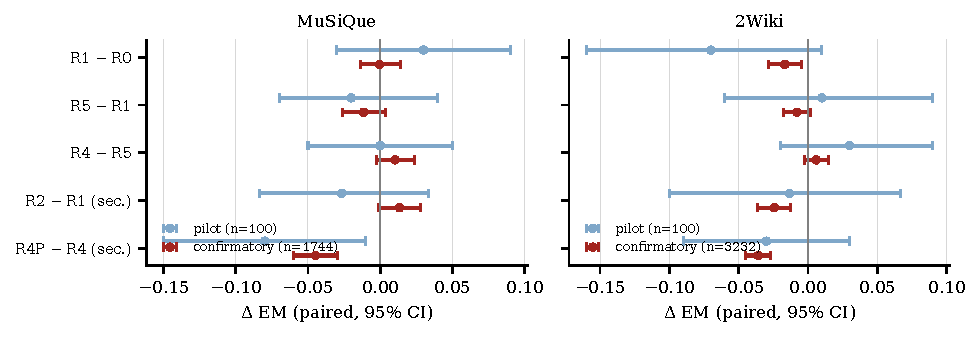
\includegraphics[width=0.92\textwidth]{figures/fig5_contrasts_pilot_vs_confirmatory.pdf}
\caption{Protocol~A contrasts in the exploratory pilot ($n$=100 per dataset) and on the disjoint confirmatory sample. The pilot estimate of R1$-$R0 on 2WikiMultiHopQA ($-0.07$) overstated the confirmed effect ($-0.017$). Contrasts marked \emph{sec.} are secondary.}
\label{fig:forest}
\end{figure*}


\subsection{Exploratory pilot results}

Protocol~B, the retrieved-evidence baselines and the perturbations were run only on the exploratory pilot ($n=100$ per primary dataset). Appendix~\ref{app:pilot} gives the details and Appendix~\ref{app:tables} the tables. \emph{Budget (Protocol~B).} Under a budget equal to the content tokens of the fact set, with each representation keeping as much of the shared ranking as it can afford, R0 keeps 0.83 (2WikiMultiHopQA) and 0.81 (MuSiQue) of the facts, against 0.62--0.65 for R1, R4 and R5, whose identifiers, titles and relation lines cost 2.5 to 4 times as many overhead tokens. The answer string consequently remains in 0.85 of R0 blocks on 2WikiMultiHopQA but only 0.64--0.66 of the others; the accuracy differences are smaller than these losses and inconclusive at this $n$. \emph{Retrieved evidence (Experiment~0).} Extracted claims and predicted paths are indistinguishable from reranked passages in exact match, at about three times the tokens. Our EG-RAG reconstruction, at a similar token count to reranked passages, is less accurate ($-0.15$ on 2WikiMultiHopQA and $-0.09$ on MuSiQue), because its budgeted selection keeps the answer string less often and it abstains more. \emph{Perturbations (Experiment~2).} Removing required facts mainly raises abstention, hard distractors lower exact match in every QA cell (by up to 0.16), and retyping 40\% of the derived relations lowers 2WikiMultiHopQA exact match by 0.10 $[-0.18, -0.01]$. Reordering and stripping titles have small effects of inconsistent sign.

\section{Discussion}
\label{sec:analysis}

\paragraph{Reorganising the same facts changed little.}
With the facts held fixed, neither the graph-derived order nor explicit derived relation lines changed exact match by more than about one point, for either reader. Gains attributed to graph-structured evidence in system-level comparisons are thus unlikely to come from relation lines or ordering as such.

\paragraph{When structure hurts: asserted contradictions.}
The clearest and only confirmed harm came from relation lines that assert a conflict. Gold supporting passages are, by construction, consistent evidence for one answer, yet the NLI classifier marks at least one pair as contradictory in 34--63\% of prompts. The interventions show that the word itself does the damage: relabelling these lines, or blanking them while keeping their number and length, recovers the loss, and nothing else about the predicted block matters measurably. The effect held prospectively on untouched questions and a new dataset, and for a second model family; the cost of sentence items, by contrast, was reader-specific (for Mistral it was null or positive). Complementing \citet{nishida-etal-2026-dissecting}, who show that noisy relations hurt GraphRAG through retrieval, they also hurt when merely displayed next to fixed, correct evidence. Automatic triage suggests most such pairs are false (40\% concern different entities, 20\% different dates), but we establish only the cost of \emph{showing} an asserted contradiction; whether it requires falsity awaits human labels.

\paragraph{Abstention is the main channel, not the only one.}
Most effects ran through the reader's willingness to answer, but asserted contradictions also produced wrong answers on fresh questions, and removing the abstention option is no remedy (12--19 more points of wrong answers). Accuracy alone conflates caution with reasoning failures; we recommend reporting outcome transitions for any comparison of evidence formats.

\section{Conclusion}
\label{sec:conclusion}

For one 7B instruction-tuned reader on MuSiQue and 2WikiMultiHopQA, a pre-registered test on 4{,}976 held-out questions found that, with the facts held fixed, graph-derived ordering and explicit derived relations did not change exact match detectably, while sentence items lowered 2WikiMultiHopQA exact match by 1.7 points through abstention. Structure hurt when it was noisy: predicted relations cost four to five points, concentrated where the predictor asserted contradictions between compatible facts. Replicating this with other generators, with human-verified relations, and with retrieved rather than gold evidence are the most useful next steps.

\section*{Limitations}
\label{sec:limitations}

\paragraph{One generator.} All results come from Qwen2.5-7B-Instruct with greedy decoding and one prompt template. The abstention behaviour that carries most of our effects is a property of this model and this prompt, which explicitly allows the answer \emph{insufficient evidence}. Larger models, other families, or a prompt without an abstention option may respond differently to the same representations. The confirmatory sample is disjoint from the pilot, but it is not an independent replication with a different generator, dataset or team.

\paragraph{Derived, not verified, structure.} Every dependency edge was derived from dataset annotations by rule. For a substantial fraction of questions the claim-level endpoint is a fallback guess; this is the stratum C of our reports, and we report contrasts per stratum, but we never treat it as gold. A 50-question human verification package was prepared but not completed, so no result concerns human-verified structure. For the same reason we did not run the component-attribution experiment (Experiment~3), which requires verified structure to be meaningful, and we report no relation precision or recall as a measure of relation quality.

\paragraph{Gold evidence.} The controlled experiments start from the gold supporting passages. This isolates representation from retrieval, but it means our null results for structure concern the case in which the facts are complete. Experiment~0 covers retrieved evidence only at pilot scale ($n=100$ per dataset).

\paragraph{Pilot-scale secondary results.} Protocol~B, the perturbation experiment, the retrieval baselines and the secondary datasets were run only on the exploratory pilot. Many of their comparisons are underpowered, and they involve many cells, so individual intervals that exclude zero should not be over-interpreted. The pilot overestimated the one effect that we later confirmed by a factor of four.

\paragraph{Metric.} Exact match is strict. A manual check found near-misses such as missing diacritics and partial titles, and folding diacritics as a secondary check changed few records and no conclusion. Coverage and token F1 are reported alongside it. The NLI-based groundedness metric gave very low values even on unperturbed evidence, and we do not interpret it.

\paragraph{Analyses added after the confirmatory result.} The abstention decomposition and the analysis of predicted contradiction lines were designed after we saw the confirmatory result. They explain the mechanism of effects that were measured independently, but they are exploratory.

\paragraph{Unexecuted experiments.} Temporal-conflict perturbations (P7) need verified temporal data, which do not exist for these datasets. Experiment~3 needs verified structure. An adaptive representation selector (Experiment~4) is not evaluated: our results show no representation property that predicts a consistent accuracy gain, so there was nothing for a selector to exploit.

\paragraph{Compute and hardware.} All generations ran on a single 32\,GB GPU with batch size~1, using about 10 GPU-hours in total. We did not explore sampling-based decoding or multiple seeds of the generator.


\bibliography{references}

\appendix

\section{Pipeline and prompts}
\label{app:prompts}

\begin{figure*}[t]
\centering
\resizebox{\textwidth}{!}{% Figure 1: evidence pipeline (schematic; contains no numbers).
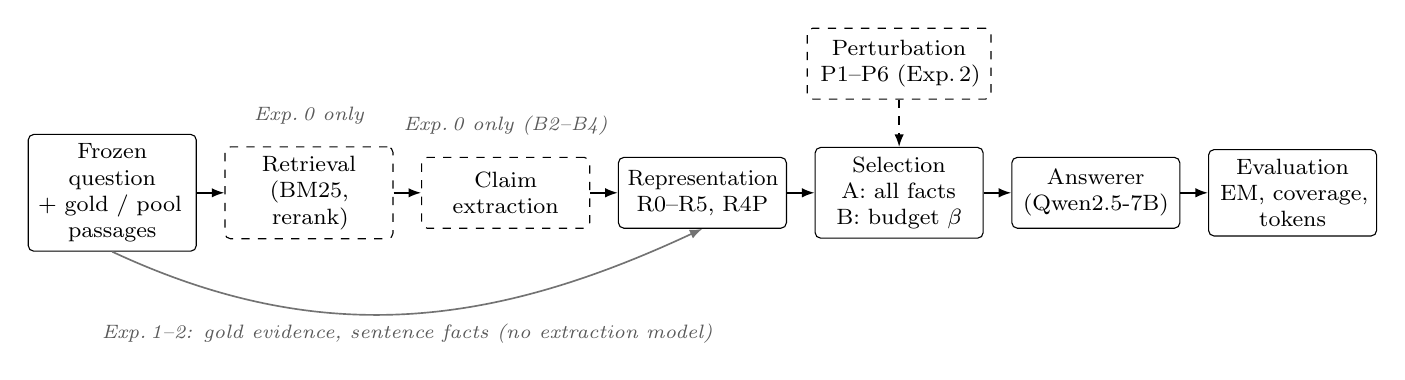
\begin{tikzpicture}[
  font=\footnotesize,
  box/.style={draw, rounded corners=2pt, align=center, minimum height=9mm, text width=19mm, fill=white},
  opt/.style={box, dashed},
  exp/.style={font=\scriptsize\itshape, text=black!65, align=center},
  arr/.style={-{Latex[length=1.6mm]}, semithick},
  node distance=3.5mm and 3.5mm]
\node[box] (data) {Frozen question\\+ gold / pool passages};
\node[opt, right=of data] (ret) {Retrieval\\(BM25, rerank)};
\node[opt, right=of ret] (ext) {Claim\\extraction};
\node[box, right=of ext] (rep) {Representation\\R0--R5, R4P};
\node[box, right=of rep] (sel) {Selection\\A: all facts\\B: budget $\beta$};
\node[box, right=of sel] (gen) {Answerer\\(Qwen2.5-7B)};
\node[box, right=of gen] (ev) {Evaluation\\EM, coverage,\\tokens};
\draw[arr] (data) -- (ret); \draw[arr] (ret) -- (ext); \draw[arr] (ext) -- (rep);
\draw[arr] (rep) -- (sel); \draw[arr] (sel) -- (gen); \draw[arr] (gen) -- (ev);
\draw[arr, black!55] (data.south) to[out=-25, in=-155] node[exp, below, pos=0.5] {Exp.\,1--2: gold evidence, sentence facts (no extraction model)} (rep.south);
\node[opt, above=6mm of sel, text width=21mm] (pert) {Perturbation\\P1--P6 (Exp.\,2)};
\draw[arr, dashed] (pert) -- (sel);
\node[exp, above=1.5mm of ext] {Exp.\,0 only (B2--B4)};
\node[exp, above=1.5mm of ret] {Exp.\,0 only};
\end{tikzpicture}
}
\caption{The evidence pipeline. Experiment~1 starts from the gold passages and varies only the representation (Protocol~A), or the representation under a fixed fact ranking and token budget (Protocol~B). Experiment~0 runs the retrieved-evidence pipeline for five systems; Experiment~2 corrupts the evidence of two representations. Dashed boxes are used only by some conditions.}
\label{fig:pipeline}
\end{figure*}


Every Experiment~0--2 answer uses the same prompt (version \texttt{qa-v2}); only the evidence block differs between representations. The system message is \emph{You answer using only the evidence you are given.} The user message is:

\begin{footnotesize}
\begin{verbatim}
Use only the evidence below to answer the question.
Each evidence item has an ID such as [E1]. Items may
be grouped into steps or followed by a list of
relations between items.

Evidence:
{evidence}

Question: {question}

Reply in exactly two lines:
Answer: <short answer: a name, date, number, short
phrase, or yes/no>
Evidence: <IDs of the items you used, e.g. E1, E2>
If the evidence is not sufficient, reply
"Answer: insufficient evidence".
\end{verbatim}
\end{footnotesize}

\noindent The assistant turn is prefilled with \texttt{Answer:}. HoVer and FEVER use the same template with \emph{Claim} in place of \emph{Question}, ask for one of the dataset's labels, and have no abstention line. The claim extractor of Experiment~0 (version \texttt{extract-v2}) uses the system message \emph{You split sentences into short, simple facts.} and asks for one fact per line, naming the subject instead of using pronouns and using only information stated in the sentence. Its output is prefilled with \texttt{- }.

\section{Serialisation examples}
\label{app:serialisation}

The following renderings are produced by the experiment code for a MuSiQue development question that was used only during prompt development and is excluded from every reported run: \emph{What character in Princess Diaries does the actress play who was also a cast member in On Golden Pond?} (gold: \emph{Queen dowager Clarisse Renaldi}). Long sentences are abbreviated here with ``\dots''.

\paragraph{R0 (passages).}
\begin{footnotesize}
\begin{verbatim}
[E1] (source: The Princess Diaries
(film)) The Princess Diaries is a 2001
American teen romantic comedy ... It
stars Anne Hathaway ... ruled by her
grandmother Queen dowager Clarisse
Renaldi (Julie Andrews). ...
[E2] (source: On Golden Pond (2001
film)) On Golden Pond is a 2001
American television adaptation of the
play starring Julie Andrews and
Christopher Plummer. ...
\end{verbatim}
\end{footnotesize}

\paragraph{R1 (sentences, dataset order).}
\begin{footnotesize}
\begin{verbatim}
[E1] (source: The Princess Diaries
(film)) The Princess Diaries is a 2001
American teen romantic comedy ...
[E2] (source: The Princess Diaries
(film)) It stars Anne Hathaway ...
Queen dowager Clarisse Renaldi (Julie
Andrews).
[E3] (source: The Princess Diaries
(film)) The film also stars ...
[E4] (source: On Golden Pond (2001
film)) On Golden Pond is a 2001
American television adaptation of the
play starring Julie Andrews and
Christopher Plummer.
[E5] ... [E6] ...
\end{verbatim}
\end{footnotesize}

\noindent Item E2 begins with a pronoun. Separated from its passage, its subject is recoverable only through the source title that every item carries. We record such context-dependent facts per question; they are one way in which an information-equivalent transformation can still change what is easy to read.

\paragraph{R3 (steps), R5 (graph order) and R4 (graph order plus relations).}
R3 groups the same six items under \texttt{Step 1:} (the three \emph{On Golden Pond} sentences) and \texttt{Step 2:} (the three \emph{Princess Diaries} sentences), following the MuSiQue decomposition. R5 lists the same items in the same order without step headers. R4 is R5 followed by
\begin{footnotesize}
\begin{verbatim}
Relations:
E5 DEPENDS_ON E1
\end{verbatim}
\end{footnotesize}
\noindent i.e.\ the sentence naming the character depends on the sentence establishing that Julie Andrews was in \emph{On Golden Pond}. This edge is derived from the MuSiQue decomposition with an exact anchor; it is not human-verified.

\section{Reconstruction of the EG-RAG baseline}
\label{app:reconstruction}

B4 follows the stage order of the EG-RAG algorithm: hybrid retrieval, reranking, claim extraction, relation prediction, belief and utility propagation, conflict resolution, budgeted subgraph selection and serialisation. Every component that the original description leaves unspecified is our choice:
\begin{itemize}
\item BM25 plus bge-small-en-v1.5 with min--max normalisation and equal weights;
\item ms-marco-MiniLM-L6-v2 reranking;
\item the 7B generator as claim extractor, with a lexical-support filter;
\item nli-deberta-v3-xsmall for support, contradiction and duplication, with thresholds 0.7 and 0.9;
\item a title-mention heuristic for dependencies;
\item years as the only temporal signal;
\item our own feature weights, a 450-token budget and at most 12 claims;
\item greedy connected selection.
\end{itemize}
The full ledger is in the repository (\texttt{docs/NOVELTY\_AND\_BASELINES.md}). B4 is therefore a reconstruction under our choices. Its results say nothing about the original implementation, and no result of the original paper is reused.

\section{Perturbations}
\label{app:perturbations}

Experiment~2 applies each intervention to the R1 and R4 renderings of the gold evidence with a recorded seed (0). The rates are $\{0.2, 0.4\}$ for P1--P4 and $0.4$ for P5 and P6, each against the same question's rate-0 record, and $k=\lceil \text{rate}\cdot n_{\text{eligible}}\rceil$ items are affected.
\begin{itemize}
\item \textbf{P1} removes required (gold-support) facts.
\item \textbf{P2} retypes or flips derived relations (R4 only).
\item \textbf{P3} permutes item positions.
\item \textbf{P4} inserts real non-gold sentences from the question's own candidate pool, chosen by BM25 similarity (\emph{hard}), and never sentences containing a gold answer.
\item \textbf{P5} strips source titles.
\item \textbf{P6} deletes a negation, or replaces an entity in a fact with \emph{it}.
\end{itemize}
Every changed item is recorded before and after. P1 and P6 can remove the answer and are therefore not label-preserving; we report their answer-change and abstention rates but no accuracy change. An intervention is unavailable when nothing is eligible:
\begin{itemize}
\item P2 on R1 or on questions without edges;
\item P3 with a single item;
\item P4 on HoVer and FEVER, which have no candidate pool;
\item P6 when no fact contains a negation;
\item P7 everywhere, since no verified temporal data exist.
\end{itemize}
These cases are counted and never scored as zero.

\section{Details of the exploratory pilot results}
\label{app:pilot}

\paragraph{Evidence loss under a token budget (pilot).}

Protocol~B was run only in the exploratory pilot (Figure~\ref{fig:budget} and Table~\ref{tab:budget}, Appendix~\ref{app:tables}). Its accounting of what each condition showed is deterministic and does not depend on the generator. Under a budget equal to the content tokens of the fact set, with each representation keeping as much of the shared ranking as it can afford, R0 keeps 0.83 (2WikiMultiHopQA) and 0.81 (MuSiQue) of the facts, whereas R1 keeps 0.64 and 0.65 and R4 keeps 0.63 and 0.62, because their identifiers, titles and relation lines cost 104--108 (2Wiki) and 81--88 (MuSiQue) tokens of overhead against 28 and 32 for R0. The verbose formats also lose the facts that matter: R0 drops 0.11 answer-bearing facts per question on 2WikiMultiHopQA against 0.33 for R1 and 0.34 for R4 (MuSiQue: 0.19, 0.28 and 0.35), so that the answer string remains in 0.85 of R0 blocks but only 0.66 of R1 and 0.64 of R4 blocks. The corresponding accuracy differences are smaller than these evidence losses and inconclusive at $n=100$. For example, R1$-$R0 is $-0.05$ $[-0.11, +0.01]$ on 2WikiMultiHopQA, and R4$-$R5 is $-0.05$ $[-0.11, +0.01]$ on MuSiQue. Under the shared policy, every representation shows the same facts and pays the same evidence loss. Halving the budget reduces exact match for every representation to 0.08--0.19.



\paragraph{Retrieved-evidence baselines (pilot).}

Table~\ref{tab:exp0} (Appendix~\ref{app:tables}) reports Experiment~0 on the 200 primary pilot questions. Reranking (B1) improves on BM25 (B0) on MuSiQue by $+0.06$ $[0.00, +0.12]$, and the 2WikiMultiHopQA difference is inconclusive. Extracted claims (B2) and predicted reasoning paths (B3) are indistinguishable from reranked passages in exact match; the extracted claims keep the answer string as often as the passages they come from (0.78 and 0.44), but at roughly three times the evidence tokens (1{,}390--1{,}711 against 501--538), because every passage sentence becomes several facts. Our reconstruction of EG-RAG (B4) uses a similar number of tokens to B1 (442--489 against 501--538) but is less accurate, by $-0.15$ $[-0.23, -0.07]$ on 2WikiMultiHopQA and $-0.09$ $[-0.15, -0.04]$ on MuSiQue: its budgeted selection keeps the answer string less often (0.56 against 0.78; 0.31 against 0.44), and coverage falls by 0.29 and 0.15.


\paragraph{Controlled perturbations (pilot).}

Table~\ref{tab:exp2} and Figure~\ref{fig:perturb} (Appendix~\ref{app:tables}) summarise Experiment~2. These comparisons are many (roughly fifty cells), and we expect a few intervals to exclude zero by chance; we report the patterns that recur across datasets or representations. When required facts are removed (P1), the model mostly abstains rather than guessing: abstention rises from 0.43 to 0.72 on MuSiQue (R1) and from 0.24 to 0.48 on 2WikiMultiHopQA. Hard distractors (P4) reduce exact match in every QA cell, by up to 0.16 (HotpotQA R1, $[-0.28, -0.04]$) and by 0.09 on MuSiQue R1 ($[-0.17, -0.01]$), and raise abstention on MuSiQue. Retyping or flipping 40\% of the derived relations (P2, R4 only) lowers 2WikiMultiHopQA exact match by 0.10 $[-0.18, -0.01]$ on the 71 questions that have relations, and is inconclusive on MuSiQue and HotpotQA. Reordering (P3) and stripping source titles (P5) produce small effects of inconsistent sign, and HoVer and FEVER verdicts are almost unaffected by any intervention.



On the secondary datasets (50 questions each; run \texttt{C\_exp0}), every Experiment~0 contrast is inconclusive, e.g.\ B4$-$B1 is $0.00$ $[-0.12, +0.12]$ EM on HotpotQA and $-0.06$ $[-0.22, +0.12]$ verdict accuracy on HoVer.

\section{Additional results}
\label{app:tables}

Table~\ref{tab:absolute} gives the absolute scores of every representation under Protocol~A in the expanded pilot, Table~\ref{tab:budget} the full information accounting under Protocols~A and~B, Table~\ref{tab:exp0} the retrieved-evidence baselines, and Table~\ref{tab:exp2} and Figure~\ref{fig:perturb} the perturbation experiment. Table~\ref{tab:confirm-secondary} lists the secondary contrasts on the confirmatory sample and Table~\ref{tab:r4p} the analysis of predicted contradiction lines; the remaining tables and figures are exploratory pilot results.

\begin{table*}[t]
\centering
\small
\begin{adjustbox}{max width=\linewidth}
\begin{tabular}{@{}llrrlrr@{}}
\toprule
Data & Contrast & $n$ & $\Delta$EM & 95\% CI & Ident. & $\Delta$Cov. \\
\midrule
MuSiQue & R2$-$R1 & 1744 & +0.013 & [-0.001, +0.028] & 2 & +0.041 \\
MuSiQue & R3$-$R5 & 1744 & -0.007 & [-0.016, +0.002] & 0 & -0.015 \\
MuSiQue & R4P$-$R4 & 1744 & -0.045 & [-0.060, -0.030] & 94 & -0.089 \\
2Wiki & R2$-$R1 & 3232 & -0.024 & [-0.036, -0.012] & 4 & -0.017 \\
2Wiki & R3$-$R5 & 3232 & -0.004 & [-0.016, +0.008] & 0 & -0.015 \\
2Wiki & R4P$-$R4 & 3232 & -0.036 & [-0.045, -0.027] & 818 & -0.061 \\
\bottomrule
\end{tabular}
\end{adjustbox}
\caption{Secondary contrasts on the confirmatory sample (pre-specified as secondary; not part of the tested family, so descriptive). Source: \texttt{F\_exp1\_contrasts.csv}.}
\label{tab:confirm-secondary}
\end{table*}

\begin{table*}[t]
\centering
\footnotesize
\begin{adjustbox}{max width=\linewidth}
\begin{tabular}{@{}llrrrrr@{}}
\toprule
Data & Contrast & $\Delta$EM & both ans. & one abstains & abst.\ only first / only second & neither \\
\midrule
2Wiki & R1$-$R0 & -0.017 & +0.001 & -0.018 & 250/81 & 529 \\
2Wiki & R4$-$R5 & +0.006 & +0.010 & -0.004 & 123/88 & 731 \\
2Wiki & R4P$-$R4 & -0.036 & -0.011 & -0.025 & 257/59 & 795 \\
2Wiki & R5$-$R1 & -0.008 & -0.004 & -0.004 & 170/130 & 649 \\
MuSiQue & R1$-$R0 & -0.001 & -0.002 & +0.001 & 94/110 & 710 \\
MuSiQue & R4$-$R5 & +0.010 & +0.006 & +0.004 & 82/89 & 709 \\
MuSiQue & R4P$-$R4 & -0.045 & -0.005 & -0.040 & 218/63 & 728 \\
MuSiQue & R5$-$R1 & -0.011 & -0.012 & +0.001 & 98/104 & 700 \\
\bottomrule
\end{tabular}
\end{adjustbox}
\caption{Exploratory decomposition of each paired EM difference on the confirmatory sample (added after the confirmatory result). \emph{both ans.}: contribution of questions answered under both representations; \emph{one abstains}: contribution of questions answered under only one. The columns sum to $\Delta$EM. Source: \texttt{F\_exp1\_decomposition\_exploratory.csv}.}
\label{tab:decomposition}
\end{table*}

\begin{table}[t]
\centering
\footnotesize
\begin{tabular}{@{}lcrrrrr@{}}
\toprule
Data & R4P shows CONTRADICTS & $n$ & Abst.\ R4 & Abst.\ R4P & EM R4 & EM R4P \\
\midrule
2Wiki & yes & 2034 & 0.32 & 0.41 & 0.33 & 0.28 \\
2Wiki & no & 1198 & 0.17 & 0.17 & 0.48 & 0.48 \\
MuSiQue & yes & 1010 & 0.50 & 0.63 & 0.25 & 0.18 \\
MuSiQue & no & 734 & 0.39 & 0.42 & 0.33 & 0.32 \\
\bottomrule
\end{tabular}
\caption{Exploratory: the same questions under derived relations (R4) and predicted relations (R4P), split by whether the predicted block contains at least one \texttt{CONTRADICTS} line (an input property). Source: \texttt{F\_exp1\_r4p\_relations\_exploratory\_paired.csv}.}
\label{tab:r4p}
\end{table}

\begin{table*}[t]
\centering
\footnotesize
\begin{tabular}{@{}lccccccc@{}}
\toprule
Data & R0 & R1 & R2 & R3 & R4 & R4P & R5 \\
\midrule
MuSiQue & 0.28 (0.57) & 0.31 (0.57) & 0.28 (0.59) & 0.24 (0.52) & 0.29 (0.59) & 0.21 (0.42) & 0.29 (0.58) \\
2Wiki & 0.44 (0.84) & 0.37 (0.76) & 0.36 (0.74) & 0.37 (0.67) & 0.41 (0.69) & 0.38 (0.66) & 0.38 (0.70) \\
HotpotQA & 0.40 (0.88) & 0.42 (0.82) & 0.35 (0.85) & 0.40 (0.86) & 0.40 (0.84) & 0.42 (0.80) & 0.38 (0.82) \\
HoVer & 0.68 (1.00) & 0.68 (1.00) & 0.73 (1.00) & -- & 0.68 (1.00) & 0.74 (1.00) & 0.68 (1.00) \\
FEVER & 0.96 (1.00) & 0.96 (1.00) & 0.97 (1.00) & -- & 0.96 (1.00) & 0.96 (1.00) & 0.96 (1.00) \\
\bottomrule
\end{tabular}
\caption{Exploratory pilot, Protocol~A: EM (QA) or verdict accuracy (HoVer, FEVER), with coverage (answered rate) in parentheses, for the same facts in seven representations. $n$=100 (MuSiQue, 2Wiki) or 50. R3 is unavailable without a reasoning order. Source: \texttt{C\_exp1\_absolute.csv}.}
\label{tab:absolute}
\end{table*}

\begin{table*}[t]
\centering
\footnotesize
\begin{tabular}{@{}lllrrrrrrr@{}}
\toprule
Data & Setting & Rep. & Kept & Ovh. & Tok. & Ans.\ drop & Ans.\ in ev. & EM & Cov. \\
\midrule
MuSiQue & A & R0 & 1.00 & 33 & 378 & 0.00 & 0.99 & 0.28 & 0.57 \\
MuSiQue & A & R1 & 1.00 & 122 & 467 & 0.00 & 0.99 & 0.31 & 0.57 \\
MuSiQue & A & R5 & 1.00 & 122 & 467 & 0.00 & 0.99 & 0.29 & 0.58 \\
MuSiQue & A & R4 & 1.00 & 141 & 486 & 0.00 & 0.99 & 0.29 & 0.59 \\
MuSiQue & B 1.0$\times$ per-rep. & R0 & 0.81 & 32 & 327 & 0.19 & 0.89 & 0.25 & 0.52 \\
MuSiQue & B 1.0$\times$ per-rep. & R1 & 0.65 & 81 & 322 & 0.28 & 0.85 & 0.26 & 0.52 \\
MuSiQue & B 1.0$\times$ per-rep. & R5 & 0.65 & 81 & 322 & 0.28 & 0.85 & 0.22 & 0.53 \\
MuSiQue & B 1.0$\times$ per-rep. & R4 & 0.62 & 88 & 321 & 0.35 & 0.80 & 0.17 & 0.44 \\
MuSiQue & B 1.0$\times$ shared & R0 & 0.60 & 30 & 251 & 0.38 & 0.77 & 0.18 & 0.47 \\
MuSiQue & B 1.0$\times$ shared & R1 & 0.60 & 75 & 296 & 0.38 & 0.77 & 0.20 & 0.48 \\
MuSiQue & B 1.0$\times$ shared & R5 & 0.60 & 75 & 296 & 0.38 & 0.77 & 0.18 & 0.52 \\
MuSiQue & B 1.0$\times$ shared & R4 & 0.60 & 86 & 307 & 0.38 & 0.77 & 0.17 & 0.46 \\
MuSiQue & B 0.5$\times$ per-rep. & R0 & 0.34 & 23 & 144 & 0.71 & 0.49 & 0.10 & 0.30 \\
MuSiQue & B 0.5$\times$ per-rep. & R1 & 0.30 & 38 & 143 & 0.77 & 0.43 & 0.09 & 0.30 \\
MuSiQue & B 0.5$\times$ per-rep. & R5 & 0.30 & 38 & 143 & 0.77 & 0.43 & 0.09 & 0.30 \\
MuSiQue & B 0.5$\times$ per-rep. & R4 & 0.29 & 39 & 142 & 0.79 & 0.42 & 0.08 & 0.31 \\
MuSiQue & B 0.5$\times$ shared & R0 & 0.27 & 21 & 120 & 0.80 & 0.42 & 0.09 & 0.28 \\
MuSiQue & B 0.5$\times$ shared & R1 & 0.27 & 35 & 133 & 0.80 & 0.42 & 0.09 & 0.30 \\
MuSiQue & B 0.5$\times$ shared & R5 & 0.27 & 35 & 133 & 0.80 & 0.42 & 0.09 & 0.30 \\
MuSiQue & B 0.5$\times$ shared & R4 & 0.27 & 38 & 136 & 0.80 & 0.42 & 0.08 & 0.30 \\
\midrule
2Wiki & A & R0 & 1.00 & 29 & 414 & 0.00 & 0.98 & 0.44 & 0.84 \\
2Wiki & A & R1 & 1.00 & 157 & 543 & 0.00 & 0.98 & 0.37 & 0.76 \\
2Wiki & A & R5 & 1.00 & 157 & 543 & 0.00 & 0.98 & 0.38 & 0.70 \\
2Wiki & A & R4 & 1.00 & 167 & 552 & 0.00 & 0.98 & 0.41 & 0.69 \\
2Wiki & B 1.0$\times$ per-rep. & R0 & 0.83 & 28 & 366 & 0.11 & 0.85 & 0.38 & 0.78 \\
2Wiki & B 1.0$\times$ per-rep. & R1 & 0.64 & 104 & 361 & 0.33 & 0.66 & 0.33 & 0.67 \\
2Wiki & B 1.0$\times$ per-rep. & R5 & 0.64 & 104 & 361 & 0.33 & 0.66 & 0.31 & 0.64 \\
2Wiki & B 1.0$\times$ per-rep. & R4 & 0.63 & 108 & 361 & 0.34 & 0.64 & 0.33 & 0.64 \\
2Wiki & B 1.0$\times$ shared & R0 & 0.60 & 26 & 265 & 0.39 & 0.60 & 0.30 & 0.67 \\
2Wiki & B 1.0$\times$ shared & R1 & 0.60 & 97 & 337 & 0.39 & 0.60 & 0.27 & 0.63 \\
2Wiki & B 1.0$\times$ shared & R5 & 0.60 & 97 & 337 & 0.39 & 0.60 & 0.27 & 0.62 \\
2Wiki & B 1.0$\times$ shared & R4 & 0.60 & 103 & 342 & 0.39 & 0.60 & 0.29 & 0.62 \\
2Wiki & B 0.5$\times$ per-rep. & R0 & 0.39 & 21 & 173 & 0.59 & 0.43 & 0.17 & 0.50 \\
2Wiki & B 0.5$\times$ per-rep. & R1 & 0.32 & 52 & 171 & 0.62 & 0.39 & 0.17 & 0.39 \\
2Wiki & B 0.5$\times$ per-rep. & R5 & 0.32 & 52 & 171 & 0.62 & 0.39 & 0.19 & 0.41 \\
2Wiki & B 0.5$\times$ per-rep. & R4 & 0.31 & 52 & 170 & 0.62 & 0.39 & 0.15 & 0.38 \\
2Wiki & B 0.5$\times$ shared & R0 & 0.29 & 20 & 131 & 0.63 & 0.38 & 0.14 & 0.45 \\
2Wiki & B 0.5$\times$ shared & R1 & 0.29 & 48 & 160 & 0.63 & 0.38 & 0.15 & 0.36 \\
2Wiki & B 0.5$\times$ shared & R5 & 0.29 & 48 & 160 & 0.63 & 0.38 & 0.16 & 0.37 \\
2Wiki & B 0.5$\times$ shared & R4 & 0.29 & 50 & 161 & 0.63 & 0.38 & 0.15 & 0.37 \\
\bottomrule
\end{tabular}
\caption{Information accounting under Protocol~A and Protocol~B (budget $\beta\times$ the content tokens of the fact set). Kept: fraction of facts shown; Ovh./Tok.: mean overhead and evidence tokens; Ans.\ drop: answer-bearing facts cut per question; Ans.\ in ev.: answer string present in the block. Source: \texttt{C\_exp1\_protocol\_accounting.csv}, \texttt{C\_exp1\_absolute.csv}.}
\label{tab:budget}
\end{table*}

\begin{table*}[t]
\centering
\footnotesize
\begin{tabular}{@{}llrlrrrrrr@{}}
\toprule
Data & Sys. & EM & 95\% CI & F1 & Cov. & Tok. & Units & Ans.\ in ev. & Lat.\,(s) \\
\midrule
MuSiQue & B0 & 0.06 & [+0.02, +0.11] & 0.10 & 0.23 & 493 & 4.0 & 0.34 & 0.36 \\
MuSiQue & B1 & 0.12 & [+0.06, +0.19] & 0.17 & 0.33 & 538 & 4.0 & 0.44 & 0.36 \\
MuSiQue & B2 & 0.13 & [+0.07, +0.20] & 0.17 & 0.36 & 1390 & 57.1 & 0.44 & 0.86 \\
MuSiQue & B3 & 0.15 & [+0.08, +0.22] & 0.18 & 0.38 & 1667 & 57.1 & 0.44 & 0.91 \\
MuSiQue & B4 & 0.03 & [+0.00, +0.07] & 0.05 & 0.18 & 442 & 11.9 & 0.31 & 0.51 \\
\midrule
2Wiki & B0 & 0.23 & [+0.16, +0.31] & 0.27 & 0.54 & 506 & 4.0 & 0.69 & 0.38 \\
2Wiki & B1 & 0.26 & [+0.18, +0.35] & 0.30 & 0.54 & 501 & 4.0 & 0.78 & 0.39 \\
2Wiki & B2 & 0.24 & [+0.16, +0.33] & 0.27 & 0.48 & 1436 & 56.4 & 0.78 & 0.67 \\
2Wiki & B3 & 0.20 & [+0.12, +0.28] & 0.24 & 0.50 & 1711 & 56.4 & 0.78 & 0.68 \\
2Wiki & B4 & 0.11 & [+0.05, +0.17] & 0.13 & 0.25 & 489 & 11.9 & 0.56 & 0.51 \\
\bottomrule
\end{tabular}
\caption{Experiment~0, retrieved evidence (exploratory, $n$=100 per dataset). Tok.: mean evidence tokens; Units: items shown; Lat.: answer-generation latency (claim extraction for B2--B4 is not included). B4 is our reconstruction of EG-RAG. Source: \texttt{A\_exp0\_absolute.csv}.}
\label{tab:exp0}
\end{table*}

\begin{table*}[t]
\centering
\footnotesize
\begin{tabular}{@{}lllrrrlrl@{}}
\toprule
Data & Rep. & Perturbation & $n$ & Lab.-pres. & $\Delta$EM & 95\% CI & Ans.\ changed & Abstention \\
\midrule
MuSiQue & R1 & P1 & 100 & 0 & -- & -- & 0.40 & 0.43$\to$0.72 \\
MuSiQue & R1 & P3 & 100 & 100 & -0.07 & [-0.13, -0.02] & 0.13 & 0.43$\to$0.44 \\
MuSiQue & R1 & P4 hard & 100 & 100 & -0.09 & [-0.17, -0.01] & 0.27 & 0.43$\to$0.51 \\
MuSiQue & R1 & P5 strip & 100 & 100 & -0.03 & [-0.08, +0.02] & 0.12 & 0.43$\to$0.41 \\
MuSiQue & R1 & P6 entity & 100 & 0 & -- & -- & 0.14 & 0.43$\to$0.50 \\
MuSiQue & R1 & P6 negation & 29 & 0 & -- & -- & 0.03 & 0.52$\to$0.55 \\
\midrule
MuSiQue & R4 & P1 & 100 & 0 & -- & -- & 0.44 & 0.41$\to$0.71 \\
MuSiQue & R4 & P2 & 100 & 100 & -0.01 & [-0.07, +0.05] & 0.24 & 0.41$\to$0.47 \\
MuSiQue & R4 & P3 & 100 & 100 & -0.03 & [-0.08, +0.02] & 0.14 & 0.41$\to$0.44 \\
MuSiQue & R4 & P4 hard & 100 & 100 & -0.08 & [-0.16, +0.00] & 0.34 & 0.41$\to$0.54 \\
MuSiQue & R4 & P5 strip & 100 & 100 & +0.00 & [-0.04, +0.04] & 0.10 & 0.41$\to$0.38 \\
MuSiQue & R4 & P6 entity & 100 & 0 & -- & -- & 0.19 & 0.41$\to$0.43 \\
MuSiQue & R4 & P6 negation & 29 & 0 & -- & -- & 0.03 & 0.48$\to$0.52 \\
\midrule
2Wiki & R1 & P1 & 100 & 0 & -- & -- & 0.43 & 0.24$\to$0.48 \\
2Wiki & R1 & P3 & 100 & 100 & +0.04 & [-0.04, +0.12] & 0.30 & 0.24$\to$0.19 \\
2Wiki & R1 & P4 hard & 100 & 100 & -0.04 & [-0.13, +0.05] & 0.35 & 0.24$\to$0.31 \\
2Wiki & R1 & P5 strip & 100 & 100 & +0.02 & [-0.03, +0.08] & 0.16 & 0.24$\to$0.18 \\
2Wiki & R1 & P6 entity & 100 & 0 & -- & -- & 0.14 & 0.24$\to$0.27 \\
2Wiki & R1 & P6 negation & 15 & 0 & -- & -- & 0.00 & 0.20$\to$0.20 \\
\midrule
2Wiki & R4 & P1 & 100 & 0 & -- & -- & 0.43 & 0.31$\to$0.51 \\
2Wiki & R4 & P2 & 71 & 71 & -0.10 & [-0.18, -0.01] & 0.44 & 0.35$\to$0.34 \\
2Wiki & R4 & P3 & 100 & 100 & -0.01 & [-0.09, +0.07] & 0.26 & 0.31$\to$0.26 \\
2Wiki & R4 & P4 hard & 100 & 100 & -0.03 & [-0.12, +0.06] & 0.35 & 0.31$\to$0.36 \\
2Wiki & R4 & P5 strip & 100 & 100 & +0.08 & [+0.01, +0.16] & 0.19 & 0.31$\to$0.26 \\
2Wiki & R4 & P6 entity & 100 & 0 & -- & -- & 0.17 & 0.31$\to$0.33 \\
2Wiki & R4 & P6 negation & 15 & 0 & -- & -- & 0.00 & 0.40$\to$0.40 \\
\midrule
HotpotQA & R1 & P1 & 50 & 0 & -- & -- & 0.36 & 0.18$\to$0.44 \\
HotpotQA & R1 & P3 & 50 & 50 & -0.06 & [-0.16, +0.04] & 0.18 & 0.18$\to$0.14 \\
HotpotQA & R1 & P4 hard & 50 & 50 & -0.16 & [-0.28, -0.04] & 0.26 & 0.18$\to$0.24 \\
HotpotQA & R1 & P5 strip & 50 & 50 & -0.02 & [-0.08, +0.04] & 0.08 & 0.18$\to$0.14 \\
HotpotQA & R1 & P6 entity & 50 & 0 & -- & -- & 0.18 & 0.18$\to$0.18 \\
HotpotQA & R1 & P6 negation & 5 & 0 & -- & -- & 0.00 & 0.20$\to$0.20 \\
\midrule
HotpotQA & R4 & P1 & 50 & 0 & -- & -- & 0.42 & 0.16$\to$0.44 \\
HotpotQA & R4 & P2 & 25 & 25 & -0.04 & [-0.24, +0.12] & 0.28 & 0.08$\to$0.16 \\
HotpotQA & R4 & P3 & 50 & 50 & -0.04 & [-0.14, +0.06] & 0.14 & 0.16$\to$0.16 \\
HotpotQA & R4 & P4 hard & 50 & 50 & -0.10 & [-0.24, +0.04] & 0.34 & 0.16$\to$0.20 \\
HotpotQA & R4 & P5 strip & 50 & 50 & +0.02 & [-0.04, +0.08] & 0.08 & 0.16$\to$0.14 \\
HotpotQA & R4 & P6 entity & 50 & 0 & -- & -- & 0.16 & 0.16$\to$0.18 \\
HotpotQA & R4 & P6 negation & 5 & 0 & -- & -- & 0.00 & 0.20$\to$0.20 \\
\bottomrule
\end{tabular}
\caption{Experiment~2 at rate 0.4 (exploratory). $\Delta$EM is computed only on label-preserving records without introduced answers (Lab.-pres.); P1 and P6 can remove the answer, so only answer-change and abstention rates are given. Source: \texttt{C\_exp2\_sensitivity.csv}.}
\label{tab:exp2}
\end{table*}

\begin{figure*}[t]
\centering
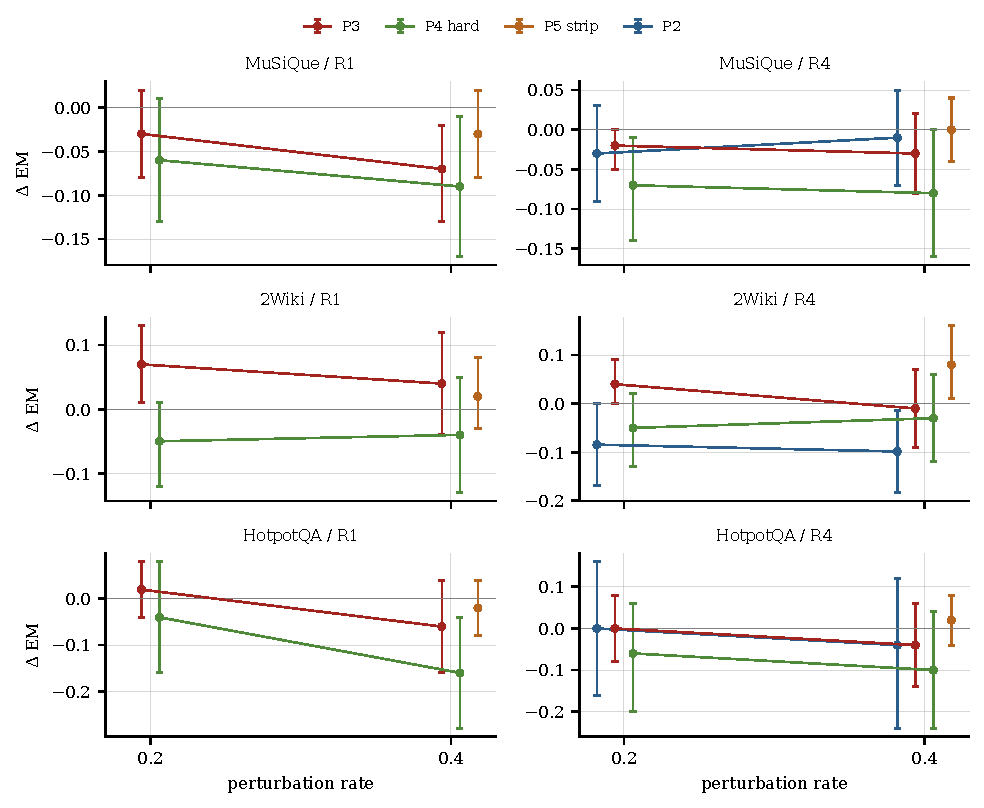
\includegraphics[width=0.8\textwidth]{figures/fig4_perturbation_sensitivity.pdf}
\caption{Exploratory pilot: change in exact match under label-preserving perturbations, relative to the same question unperturbed (95\% CIs). P1 and P6 can remove the answer and are reported in Table~\ref{tab:exp2} only.}
\label{fig:perturb}
\end{figure*}
\begin{figure*}[t]
\centering
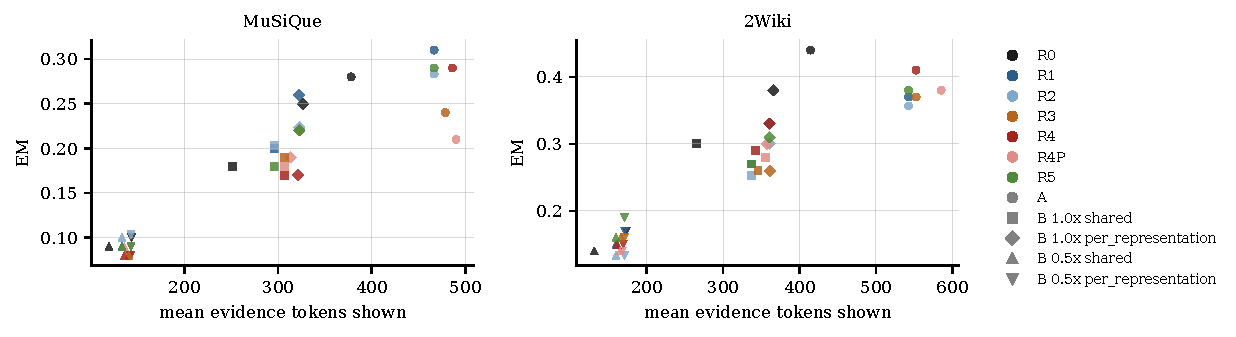
\includegraphics[width=0.85\textwidth]{figures/fig3_accuracy_vs_tokens.pdf}
\caption{Exploratory pilot: exact match against the mean number of evidence tokens shown, for Protocol~A (natural length) and Protocol~B (budget $1.0\times$ or $0.5\times$ the content tokens; shared or per-representation policy).}
\label{fig:budget}
\end{figure*}

\section{Revision experiments: supplementary tables}
\label{app:revision}

Table~\ref{tab:controls-strata} stratifies the contradiction-line effect by the number of such lines. Table~\ref{tab:contra-triage} summarises the predicted contradictions. Table~\ref{tab:retrieval} gives the retrieved-evidence contrasts under both protocols, and Table~\ref{tab:retrieval-strata} by retrieval outcome. Table~\ref{tab:exp0-costs} makes the budgets and costs of Experiment~0 explicit. All of these are exploratory. The blinded human-verification packages and their importers are described in the repository (\texttt{docs/REMAINING\_HUMAN\_VERIFICATION.md}).

\begin{table*}[t]
\centering
\footnotesize
\begin{adjustbox}{max width=\linewidth}
\begin{tabular}{@{}llrrrrlrrr@{}}
\toprule
Data & Change (second vs.\ first) & $n$ & $\Delta$EM & $\Delta$Abst. & $\Delta$Wrong & $\Delta$Acc.\ | both answered & C$\to$A / A$\to$C & C$\to$W / W$\to$C & W$\to$A / A$\to$W \\
\midrule
2Wiki & sentence items vs.\ passages & 3232 & -0.017 & +0.052 & -0.036 & +0.002 [-0.013, +0.017] & 87/29 & 152/156 & 163/52 \\
2Wiki & graph order vs.\ dataset order & 3232 & -0.008 & +0.012 & -0.004 & -0.006 [-0.018, +0.005] & 57/45 & 95/81 & 113/85 \\
2Wiki & derived relation lines vs.\ none & 3232 & +0.006 & +0.011 & -0.017 & +0.014 [+0.005, +0.024] & 42/29 & 42/74 & 81/59 \\
2Wiki & R4P vs.\ R4 (original) & 3232 & -0.036 & +0.061 & -0.025 & -0.017 [-0.027, -0.007] & 97/17 & 80/44 & 160/42 \\
2Wiki & contradiction lines on vs.\ off & 3232 & -0.033 & +0.061 & -0.028 & -0.013 [-0.022, -0.004] & 89/9 & 64/36 & 137/20 \\
\midrule
MuSiQue & sentence items vs.\ passages & 1744 & -0.001 & -0.009 & +0.010 & -0.004 [-0.020, +0.014] & 42/44 & 29/26 & 52/66 \\
MuSiQue & graph order vs.\ dataset order & 1744 & -0.011 & -0.003 & +0.015 & -0.025 [-0.045, -0.006] & 45/46 & 43/22 & 53/58 \\
MuSiQue & derived relation lines vs.\ none & 1744 & +0.010 & -0.004 & -0.006 & +0.013 [-0.007, +0.031] & 28/35 & 29/40 & 54/54 \\
MuSiQue & R4P vs.\ R4 (original) & 1744 & -0.045 & +0.089 & -0.044 & -0.012 [-0.037, +0.011] & 93/24 & 43/34 & 125/39 \\
MuSiQue & contradiction lines on vs.\ off & 1744 & -0.033 & +0.062 & -0.029 & -0.009 [-0.020, +0.003] & 52/2 & 14/7 & 64/6 \\
\bottomrule
\end{tabular}
\end{adjustbox}
\caption{Question-level outcome transitions (C correct, W answered and wrong, A not answered) between paired conditions on the confirmatory questions (exploratory decomposition). $\Delta$Acc.\ | both answered: accuracy difference among questions answered under both conditions, with 95\% CI. Sources: \texttt{revision/\allowbreak analysis/\allowbreak F\_exp1\_transitions.csv}, \texttt{revision/\allowbreak controls/\allowbreak controls\_transitions.csv}.}
\label{tab:transitions}
\end{table*}

\begin{figure*}[t]
\centering
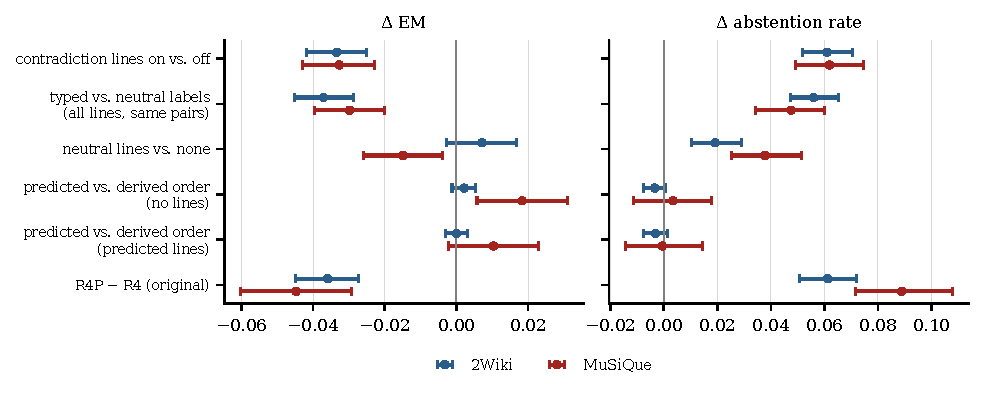
\includegraphics[width=0.9\textwidth]{figures/fig_controls.pdf}
\caption{Fixed-order relation controls on the confirmatory questions (exploratory). Each row changes one factor on identical facts; points are paired differences with 95\% CIs.}
\label{fig:controls}
\end{figure*}
\begin{table*}[t]
\centering
\footnotesize
\begin{adjustbox}{max width=\linewidth}
\begin{tabular}{@{}llrrlrl@{}}
\toprule
Data & Contradiction lines & $n$ & $\Delta$EM & 95\% CI & $\Delta$Abst. & 95\% CI \\
\midrule
2Wiki & 0 & 1198 & +0.000 & [+0.000, +0.000] & +0.000 & [+0.000, +0.000] \\
2Wiki & 1-2 & 1015 & -0.069 & [-0.089, -0.049] & +0.088 & [+0.068, +0.108] \\
2Wiki & 3-5 & 577 & -0.050 & [-0.075, -0.024] & +0.137 & [+0.106, +0.166] \\
2Wiki & 6+ & 442 & -0.020 & [-0.043, +0.002] & +0.066 & [+0.034, +0.097] \\
\midrule
MuSiQue & 0 & 734 & +0.000 & [+0.000, +0.000] & +0.000 & [+0.000, +0.000] \\
MuSiQue & 1-2 & 660 & -0.053 & [-0.073, -0.033] & +0.094 & [+0.071, +0.118] \\
MuSiQue & 3-5 & 257 & -0.039 & [-0.066, -0.016] & +0.132 & [+0.089, +0.179] \\
MuSiQue & 6+ & 93 & -0.129 & [-0.194, -0.065] & +0.129 & [+0.065, +0.204] \\
\bottomrule
\end{tabular}
\end{adjustbox}
\caption{Effect of showing the predicted \texttt{CONTRADICTS} lines (R4P\_FO$-$R4P\_FO\_NC) by the number of such lines in the prompt (exploratory). With no contradiction lines the two prompts are identical. Source: \texttt{revision/\allowbreak controls/\allowbreak relation\_control\_strata.csv}.}
\label{tab:controls-strata}
\end{table*}

\begin{table*}[t]
\centering
\footnotesize
\begin{adjustbox}{max width=\linewidth}
\begin{tabular}{@{}llrrlr@{}}
\toprule
Prompt & Contrast & $n$ & $\Delta$EM & 95\% CI & $\Delta$Abst. \\
\midrule
\texttt{qa-v2} & R1$-$R0 & 1000 & -0.023 & [-0.044, -0.002] & +0.059 \\
\texttt{qa-v2} & R4P$-$R4 & 1000 & -0.036 & [-0.054, -0.020] & +0.054 \\
\texttt{noabst} & R1$-$R0 & 1000 & -0.004 & [-0.026, +0.018] & +0.002 \\
\texttt{noabst} & R4P$-$R4 & 1000 & -0.017 & [-0.035, +0.000] & +0.003 \\
prompt effect & \texttt{noabst}$-$\texttt{qa-v2} (R0) & 1000 & +0.078 & [+0.055, +0.101] & -0.196 \\
prompt effect & \texttt{noabst}$-$\texttt{qa-v2} (R1) & 1000 & +0.097 & [+0.072, +0.123] & -0.253 \\
prompt effect & \texttt{noabst}$-$\texttt{qa-v2} (R4) & 1000 & +0.109 & [+0.084, +0.135] & -0.268 \\
prompt effect & \texttt{noabst}$-$\texttt{qa-v2} (R4P) & 1000 & +0.128 & [+0.103, +0.153] & -0.319 \\
interaction & (R1$-$R0) \texttt{noabst} minus \texttt{qa-v2} & 1000 & +0.019 & [-0.006, +0.045] & -0.057 \\
interaction & (R4P$-$R4) \texttt{noabst} minus \texttt{qa-v2} & 1000 & +0.019 & [-0.001, +0.040] & -0.051 \\
\bottomrule
\end{tabular}
\end{adjustbox}
\caption{Prompt factor (exploratory, 1{,}000 confirmatory 2Wiki questions): the frozen prompt \texttt{qa-v2} and the same prompt without the line offering \emph{insufficient evidence} (\texttt{noabst}); last rows give the prompt $\times$ representation interaction. Source: \texttt{revision/\allowbreak noabst/\allowbreak noabst\_contrasts.csv}.}
\label{tab:noabst}
\end{table*}

\begin{table*}[t]
\centering
\footnotesize
\begin{adjustbox}{max width=\linewidth}
\begin{tabular}{@{}lrr@{}}
\toprule
Automatic triage (heuristic, not a judgement) & Pairs & Share \\
\midrule
different source titles (different entities) & 3,857 & 40\% \\
same title, different years & 1,962 & 20\% \\
same title, different numbers & 671 & 7\% \\
same title, pronoun-initial sentence & 734 & 8\% \\
same title, other & 2,526 & 26\% \\
\midrule
all predicted contradiction pairs & 9,750 & 100\% \\
\bottomrule
\end{tabular}
\end{adjustbox}
\caption{Predicted \texttt{CONTRADICTS} pairs on the confirmatory sample (R4P; 12,816 directed edges, 12,372 rendered, 3,044 questions). NLI confidence $\geq$0.90 (median 0.985). Categories are heuristic triage for prioritising human verification. Source: \texttt{revision/\allowbreak contradictions/\allowbreak contradictions\_summary.json}.}
\label{tab:contra-triage}
\end{table*}

\begin{table*}[t]
\centering
\footnotesize
\begin{adjustbox}{max width=\linewidth}
\begin{tabular}{@{}lllrrrlrr@{}}
\toprule
Data & Prot. & Contrast & $n$ & Ident. & $\Delta$EM & 95\% CI & $\Delta$Abst. & Tokens \\
\midrule
MuSiQue & A & R1$-$R0 & 500 & 0 & +0.014 & [+0.000, +0.028] & -0.006 & 526$\to$653 \\
MuSiQue & A & R5$-$R1 & 500 & 451 & +0.010 & [+0.000, +0.020] & -0.008 & 653$\to$653 \\
MuSiQue & A & R4$-$R5 & 500 & 342 & +0.002 & [-0.012, +0.016] & -0.002 & 653$\to$657 \\
MuSiQue & A & R4P$-$R4 & 500 & 72 & -0.036 & [-0.056, -0.020] & +0.068 & 657$\to$701 \\
MuSiQue & A & contradiction lines on$-$off & 500 & 131 & -0.022 & [-0.038, -0.008] & +0.040 & 665$\to$701 \\
MuSiQue & A & R4P\_FO$-$R5 & 500 & 86 & -0.022 & [-0.038, -0.008] & +0.052 & 653$\to$701 \\
MuSiQue & B 1.0$\times$ & R1$-$R0 & 500 & 3 & +0.022 & [+0.002, +0.042] & +0.014 & 462$\to$457 \\
MuSiQue & B 1.0$\times$ & R5$-$R1 & 500 & 459 & +0.002 & [-0.004, +0.008] & -0.002 & 457$\to$457 \\
MuSiQue & B 1.0$\times$ & R4$-$R5 & 500 & 370 & +0.006 & [-0.004, +0.018] & -0.006 & 457$\to$457 \\
MuSiQue & B 1.0$\times$ & R4P$-$R4 & 500 & 133 & -0.032 & [-0.050, -0.016] & +0.052 & 457$\to$452 \\
MuSiQue & B 1.0$\times$ & contradiction lines on$-$off & 500 & 201 & -0.016 & [-0.028, -0.006] & +0.026 & 455$\to$452 \\
MuSiQue & B 1.0$\times$ & R4P\_FO$-$R5 & 500 & 144 & -0.020 & [-0.038, -0.004] & +0.038 & 457$\to$452 \\
\midrule
2Wiki & A & R1$-$R0 & 500 & 5 & -0.026 & [-0.054, +0.002] & +0.072 & 525$\to$681 \\
2Wiki & A & R5$-$R1 & 500 & 498 & +0.000 & [+0.000, +0.000] & +0.000 & 681$\to$681 \\
2Wiki & A & R4$-$R5 & 500 & 322 & +0.010 & [-0.008, +0.028] & -0.006 & 681$\to$685 \\
2Wiki & A & R4P$-$R4 & 500 & 84 & -0.030 & [-0.054, -0.008] & +0.066 & 685$\to$749 \\
2Wiki & A & contradiction lines on$-$off & 500 & 110 & -0.024 & [-0.046, -0.004] & +0.068 & 695$\to$749 \\
2Wiki & A & R4P\_FO$-$R5 & 500 & 66 & -0.016 & [-0.042, +0.010] & +0.052 & 681$\to$749 \\
2Wiki & B 1.0$\times$ & R1$-$R0 & 500 & 23 & +0.010 & [-0.016, +0.034] & +0.030 & 454$\to$451 \\
2Wiki & B 1.0$\times$ & R5$-$R1 & 500 & 499 & +0.000 & [+0.000, +0.000] & +0.000 & 451$\to$451 \\
2Wiki & B 1.0$\times$ & R4$-$R5 & 500 & 383 & -0.002 & [-0.014, +0.010] & +0.004 & 451$\to$451 \\
2Wiki & B 1.0$\times$ & R4P$-$R4 & 500 & 157 & -0.040 & [-0.060, -0.020] & +0.054 & 451$\to$447 \\
2Wiki & B 1.0$\times$ & contradiction lines on$-$off & 500 & 195 & -0.036 & [-0.054, -0.018] & +0.044 & 451$\to$447 \\
2Wiki & B 1.0$\times$ & R4P\_FO$-$R5 & 500 & 141 & -0.044 & [-0.066, -0.022] & +0.064 & 451$\to$447 \\
\bottomrule
\end{tabular}
\end{adjustbox}
\caption{Retrieved evidence (exploratory, fresh disjoint sample of 500 questions per dataset): every representation renders the same four reranked passages; R4/R5 use annotation-derived edges restricted to retrieved sentence pairs (oracle structure on real retrieval). Protocol B: budget $1.0\times$ content tokens, per-representation policy. Source: \texttt{revision/\allowbreak retrieval/\allowbreak retrieval\_contrasts.csv}.}
\label{tab:retrieval}
\end{table*}

\begin{table*}[t]
\centering
\footnotesize
\begin{adjustbox}{max width=\linewidth}
\begin{tabular}{@{}lllrrlr@{}}
\toprule
Data & Contrast & Stratum & $n$ & $\Delta$EM & 95\% CI & $\Delta$Abst. \\
\midrule
MuSiQue & R1$-$R0 & retrieval: complete & 149 & +0.034 & [-0.007, +0.074] & -0.034 \\
MuSiQue & R1$-$R0 & retrieval: partial & 311 & +0.006 & [-0.006, +0.019] & +0.010 \\
MuSiQue & R1$-$R0 & retrieval: none & 40 & +0.000 & [+0.000, +0.000] & -0.025 \\
MuSiQue & R1$-$R0 & distractor heavy: True & 328 & +0.006 & [+0.000, +0.015] & +0.012 \\
MuSiQue & R1$-$R0 & long evidence: True & 249 & +0.012 & [-0.008, +0.032] & -0.020 \\
MuSiQue & contradiction lines on$-$off & retrieval: complete & 149 & -0.047 & [-0.094, -0.007] & +0.047 \\
MuSiQue & contradiction lines on$-$off & retrieval: partial & 311 & -0.013 & [-0.026, -0.003] & +0.039 \\
MuSiQue & contradiction lines on$-$off & retrieval: none & 40 & +0.000 & [+0.000, +0.000] & +0.025 \\
MuSiQue & contradiction lines on$-$off & distractor heavy: True & 328 & -0.012 & [-0.024, -0.003] & +0.034 \\
MuSiQue & contradiction lines on$-$off & long evidence: True & 249 & -0.016 & [-0.040, +0.004] & +0.036 \\
\midrule
2Wiki & R1$-$R0 & retrieval: complete & 262 & -0.057 & [-0.099, -0.015] & +0.080 \\
2Wiki & R1$-$R0 & retrieval: partial & 238 & +0.008 & [-0.025, +0.042] & +0.063 \\
2Wiki & R1$-$R0 & distractor heavy: True & 119 & +0.008 & [+0.000, +0.025] & +0.067 \\
2Wiki & R1$-$R0 & long evidence: True & 250 & -0.036 & [-0.072, +0.000] & +0.060 \\
2Wiki & contradiction lines on$-$off & retrieval: complete & 262 & -0.019 & [-0.050, +0.011] & +0.069 \\
2Wiki & contradiction lines on$-$off & retrieval: partial & 238 & -0.029 & [-0.055, -0.008] & +0.067 \\
2Wiki & contradiction lines on$-$off & distractor heavy: True & 119 & -0.008 & [-0.025, +0.000] & +0.050 \\
2Wiki & contradiction lines on$-$off & long evidence: True & 250 & -0.012 & [-0.040, +0.016] & +0.072 \\
\bottomrule
\end{tabular}
\end{adjustbox}
\caption{Retrieved evidence, Protocol A, by retrospective retrieval outcome (gold labels used only to stratify). Exploratory; small strata have wide intervals. Source: \texttt{revision/\allowbreak retrieval/\allowbreak retrieval\_contrasts.csv}.}
\label{tab:retrieval-strata}
\end{table*}

\begin{table*}[t]
\centering
\footnotesize
\begin{adjustbox}{max width=\linewidth}
\begin{tabular}{@{}llrrrrrrrrr@{}}
\toprule
Data & Sys. & EM & Cov. & Tok. & Units & Gold-pass.\ rec. & Ans.\ in ev. & Extr.\ calls & Latency (s) & CONTRA share \\
\midrule
MuSiQue & B0 & 0.06 & 0.23 & 493 & 4.0 & 0.44 & 0.34 & 0.0 & 0.4 & -- \\
MuSiQue & B1 & 0.12 & 0.33 & 538 & 4.0 & 0.53 & 0.44 & 0.0 & 0.4 & -- \\
MuSiQue & B2 & 0.13 & 0.36 & 1390 & 57.1 & 0.53 & 0.44 & 15.3 & 24.3 & -- \\
MuSiQue & B3 & 0.15 & 0.38 & 1667 & 57.1 & 0.53 & 0.44 & 15.3 & 24.4 & -- \\
MuSiQue & B4 & 0.03 & 0.18 & 442 & 11.9 & 0.55 & 0.31 & 15.1 & 23.8 & 0.55 \\
\midrule
2Wiki & B0 & 0.23 & 0.54 & 506 & 4.0 & 0.76 & 0.69 & 0.0 & 0.4 & -- \\
2Wiki & B1 & 0.26 & 0.54 & 501 & 4.0 & 0.80 & 0.78 & 0.0 & 0.4 & -- \\
2Wiki & B2 & 0.24 & 0.48 & 1436 & 56.4 & 0.80 & 0.78 & 14.7 & 23.9 & -- \\
2Wiki & B3 & 0.20 & 0.50 & 1711 & 56.4 & 0.80 & 0.78 & 14.7 & 23.9 & -- \\
2Wiki & B4 & 0.11 & 0.25 & 489 & 11.9 & 0.80 & 0.56 & 14.7 & 23.8 & 0.62 \\
\bottomrule
\end{tabular}
\end{adjustbox}
\caption{Experiment~0 with budgets and costs made explicit (pilot, $n$=100 per dataset). Budgets are \emph{not} matched: B2/B3 show about three times the tokens of B0/B1; B4 selects at most 12 claims within 450 tokens. Latency includes LLM claim extraction (original-call latency for cached calls). CONTRA share: fraction of B4's predicted relations labelled \texttt{CONTRADICTS}. Source: \texttt{revision/\allowbreak analysis/\allowbreak C\_exp0\_costs.csv}.}
\label{tab:exp0-costs}
\end{table*}


\begin{figure*}[t]
\centering
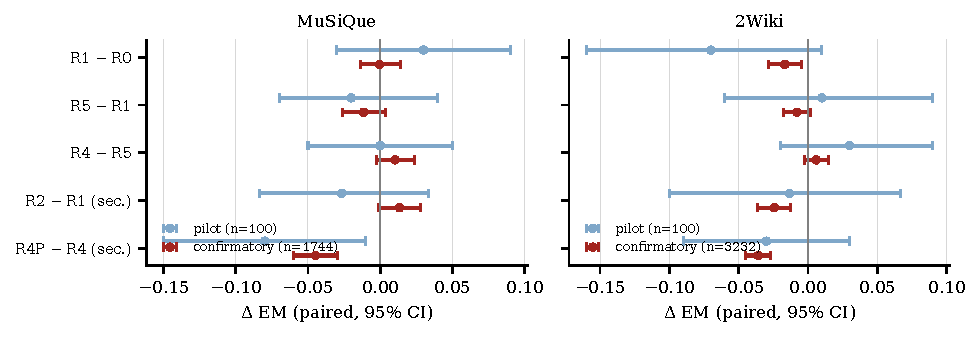
\includegraphics[width=0.85\textwidth]{figures/fig5_contrasts_pilot_vs_confirmatory.pdf}
\caption{Protocol~A contrasts in the exploratory pilot ($n$=100 per dataset) and on the disjoint confirmatory sample. The pilot estimate of R1$-$R0 on 2WikiMultiHopQA ($-0.07$) overstated the confirmed effect ($-0.017$) by a factor of four.}
\label{fig:forest}
\end{figure*}


\end{document}
